\documentclass{article}
\usepackage[UTF8]{ctex}  % 使用中文支持包
\usepackage[a4paper, margin=1in]{geometry}  % 设置纸张大小和边距
\usepackage{anyfontsize}  % 解决字体大小报错问题
\usepackage{fancyhdr}  % 设置页眉、页脚、页码
\usepackage{longtable}  % 支持长表格

\usepackage{amsmath}  % 数学公式支持
\usepackage{cases}  % 支持联立编号
\usepackage{cite}  % 引用支持

\usepackage{graphicx}  % 插入图片支持
\usepackage{float}  % 设置图片浮动位置
\usepackage{subfigure}  % 插入多图时用子图显示

\usepackage{listings}  % 代码块支持
\usepackage{xcolor}  % 设置代码块颜色

\usepackage[hyphens]{url}  % 支持链接换行
\usepackage{hyperref}  % 超链接支持
\usepackage{lastpage}  % 添加lastpage包

\usepackage{gbt7714}  %国标参考文献

\hypersetup{
    hidelinks,
    colorlinks=true,
    allcolors=black,
    pdfstartview=Fit,
    breaklinks=true
}

\title{射线源导论-第二周作业}
\author{\LaTeX\ by\ Jerry\ }
\date{\today}
\pagenumbering{arabic}

\begin{document}
\pagestyle{fancy}

\fancyhead[L]{Jerry}
\fancyhead[C]{射线源导论-第二周作业}
\fancyhead[R]{\today}
\fancyfoot[C]{Page \thepage/\pageref{LastPage}}

\section*{第二周课程作业}

\subsection*{1. 已知束流的相空间如左图所示, 假设束流不受任何外⼒或⾃场作⽤, 画出经过直线漂移距离 L=a/b 之后的相空间分布. }

如图\ref{fig:phase}所示,即为所求

\begin{figure}[ht]
    \centering
    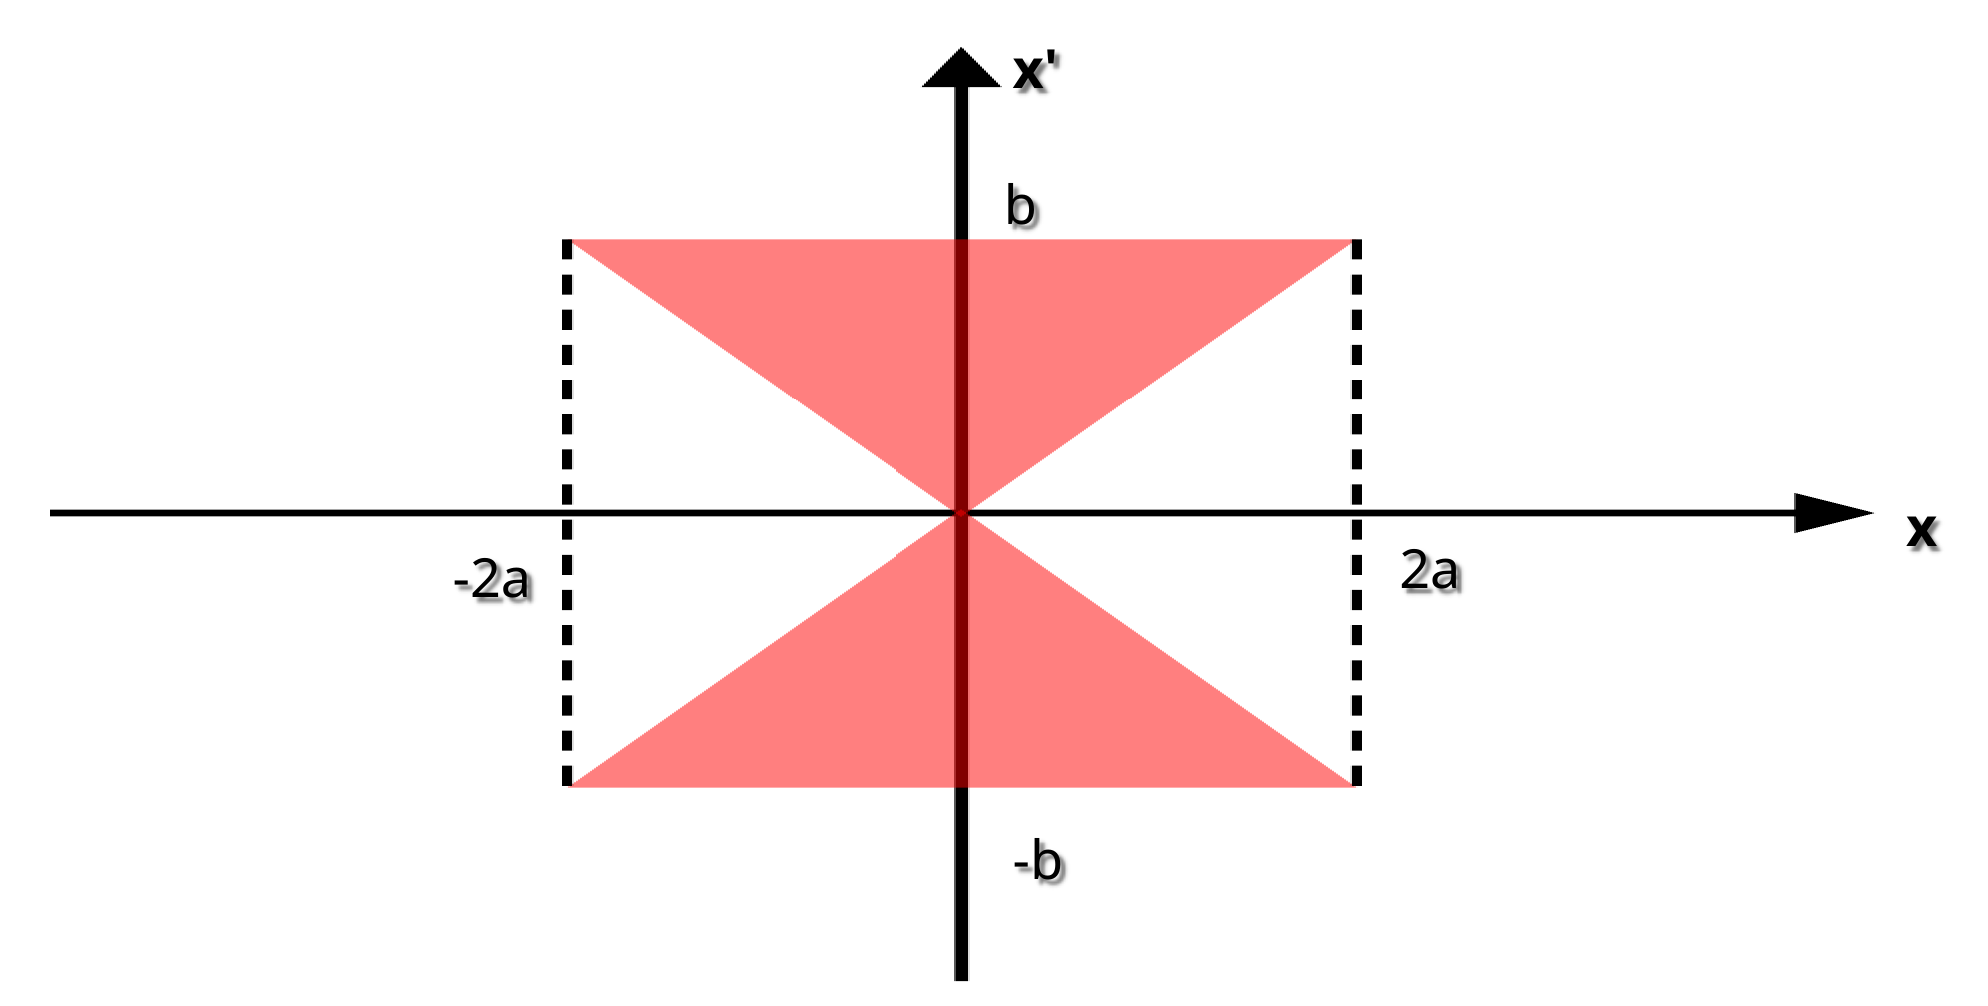
\includegraphics[width=0.8\textwidth]{img/phase.png}
    \caption{束流的相空间}
    \label{fig:phase}
\end{figure}

\subsection*{2. 画出动能为 1eV 到 10MeV 范围内的电⼦的 $\beta$ 和 $\gamma$}

速度 $\beta = v/c$ 和 $\gamma$ 之间的关系如下:

$$\beta = \sqrt{1 - \frac{1}{\gamma^2}}$$

代入动能的范围, 计算并做图得到 $\beta$ 和 $\gamma$ 的关系图如图\ref{fig:beta_gamma}所示.

\begin{figure}[ht]
    \centering
    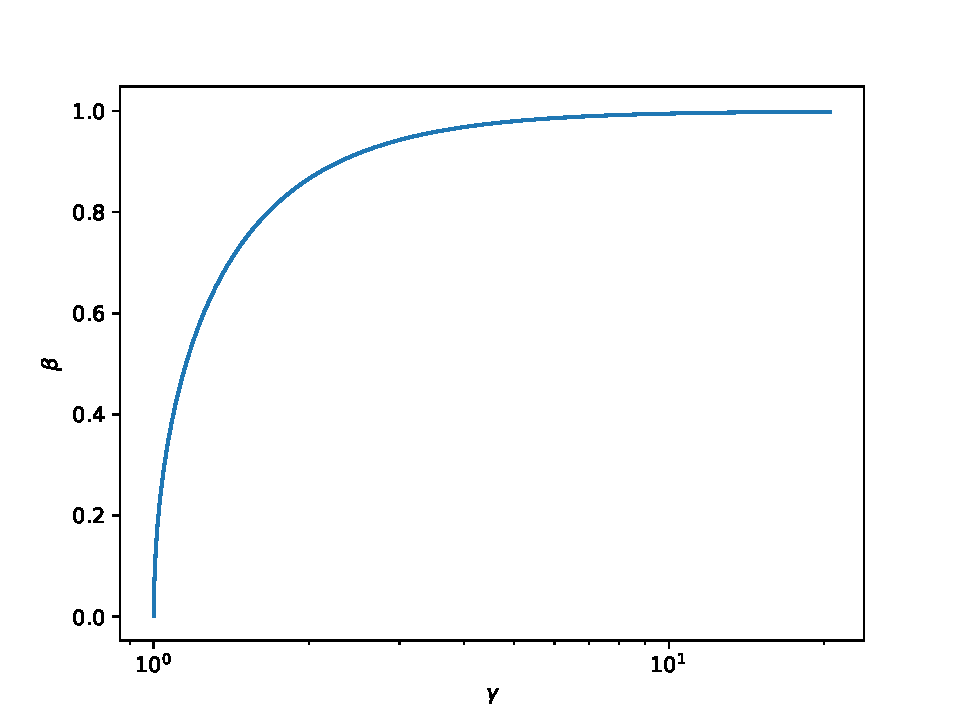
\includegraphics[width=0.8\textwidth]{img/beta_gamma.pdf}
    \caption{动能为 1eV 到 10MeV 电⼦的 $\beta$ 和 $\gamma$}
    \label{fig:beta_gamma}
\end{figure}

\subsection*{3. 计算 1eV 到 10MeV 电⼦的 de Broglie 波长}

动量计算公式:

$$p = \frac{E}{c}$$

de Broglie 波长为:

$$\lambda = \frac{h}{E/c} = \frac{hc}{E} = \frac{1240\text{eV nm}}{E}$$

代入能量 1eV 和 10MeV 计算得到 de Broglie 波长.

$$\lambda_{\text{1eV}} = 1.240 \times {10}^{3}\text{nm}, \lambda_{\text{10MeV}} = 1.240 \times {10}^{-4}\text{nm}$$

\subsection*{4. ⼀台 200keV 电镜中电流为 100pA, 计算电⼦平均纵向间距}

200keV 电子的速度为

$$ v = c \cdot  \sqrt{1 - \frac{m_e^2c_0^4}{E_e^2}} \approx 0.69531c_0 = 2.0845 \times {10}^{8} \text{m}/\text{s} $$

100pA 电流. 对电流, 有

$$ I = n \cdot e / t $$

从而

$$ n / t = I / e $$

电子的平均间距

$$ d = \frac{L}{n} = \frac{v t}{n} = \frac{v}{\frac{I}{e}} = \frac{v e}{I} $$

代入数据, 计算得到平均纵向间距

$$ d = \frac{2.0845 \times {10}^{8} \text{m}/\text{s} \times 1.6 \times {10}^{-19} \text{C}}{1\times {10}^{-10} \text{A}} = 0.33352 \text{m}$$

\subsection*{5. ⽤螺线管磁场分布和左⼿定则解释电⼦被聚焦的物理图像. 在什么情况下螺线管磁场会散焦电⼦? }

在螺线管中, Z轴方向有一个均匀磁场$B$. 如图\ref{fig:solenoid}所示.

\begin{figure}[ht]
    \centering
    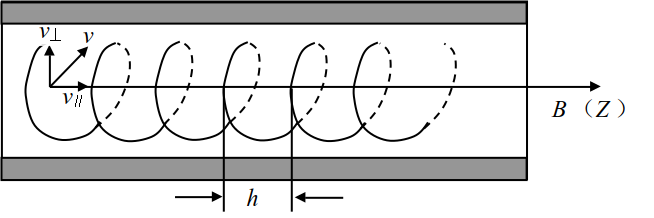
\includegraphics[width=0.6\textwidth]{img/solenoid.png}
    \caption{螺线管电子运动轨迹}
    \label{fig:solenoid}
\end{figure}

速度$v$可分解为平行$B$的分量$v_{\parallel}$和垂直于$B$的分量$v_{\perp}$, 磁场对$v_{\parallel}$分量没有作用力, $v_{\parallel}$分量使电子沿$B$方向作匀速直线运动;$v_{\perp}$分量受洛仑兹力的作用, 使电子绕$B$轴作匀速圆周运动. 因此, 电子的合成运动轨道是螺旋线, 螺旋线的半径为

$$r = \frac{m v_{\perp}}{e B}$$

其中$m$是电子的质量, $e$是电子的电荷量.

电子作圆周运动的周期为

$$ T = \frac{2\pi m}{e B} $$

可以看出, $T$与$v_{\perp}$无关, 即在同一磁场下, 不同速度的电子绕圆一周所需的时间是相等的, 只不过速度大的电子绕的圆周大, 速度小的电子绕的圆周小而已.

螺旋线的螺距为

$$ h = T v_{\parallel} = \frac{2\pi m v_{\parallel}}{e B} $$

由于$v_{\perp}$不同, 在磁场的作用下, 各电子将沿不同半径的螺旋线前进, 但由于各电子的$v_{\parallel}$分量近似相等, 所以各螺旋线的螺距是相等的. 这样, 由同一点O出发的各电子沿不同半径的螺旋线, 经过同一距离$h$后, 又重新会聚在轴线上的一点, 如图\ref{fig:magnetic_focusing}所示. 调节磁场$B$的大小, 会聚点就正好与荧光屏重合, 这就是磁聚焦.

\begin{figure}[ht]
    \centering
    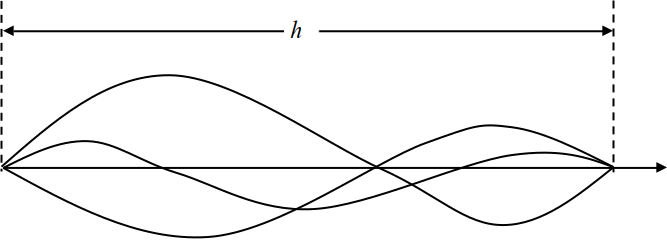
\includegraphics[width=0.5\textwidth]{img/magnetic_focusing.png}
    \caption{磁聚焦}
    \label{fig:magnetic_focusing}
\end{figure}

因此, 当会聚点与荧光屏不重合时, 电子束就会散焦. 这种情况一般发生于磁场不均匀, 导致电子无法沿着轴线聚焦.

\bibliographystyle{gbt7714-numerical}
\bibliography{cite.bib}

\end{document}
